% !ORDER = 1

\begin{problem}
求解單位長度倔強係數爲$k$, 線密度爲$\mu$的無限長線性彈簧上的一維線性波動方程
\tikzstyle{spring}=[thick, decorate,decoration={zigzag,pre length=1.5mm,post
        length=1.5mm,segment length=6}]

\begin{figure}[H]
    \centering %图片居中
    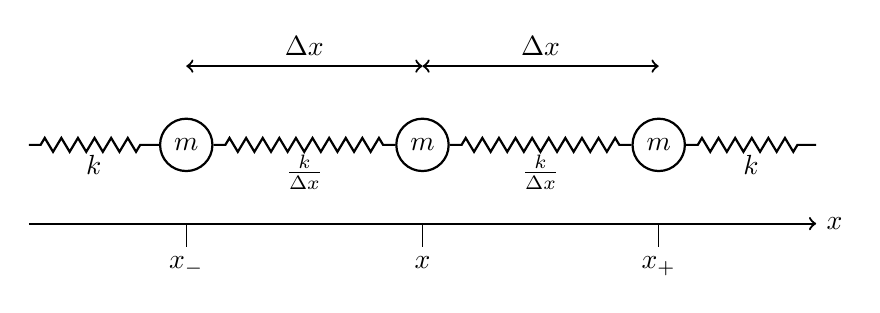
\begin{tikzpicture}
        \node[circle,draw=black,thick] (b1) at (2,0){$m$};
        \node[circle,draw=black,thick] (b2) at (5,0){$m$};
        \node[circle,draw=black,thick] (b3) at (8,0){$m$};

        \draw[spring](0,0)--(b1)node[midway,below]{$k$};
        \draw[spring](b1)--(b2)node[midway,below]{$\frac{k}{\Delta x}$};
        \draw[spring](b2)--(b3)node[midway,below]{$\frac{k}{\Delta x}$};
        \draw[spring](b3)--(10,0)node[midway,below]{$k$};

        \draw[->,thick](0,-1)--(10,-1) node[right]{$x$};
        \draw (2,-1)--(2,-1.3) node[anchor=north]{$x_-$};
        \draw (5,-1)--(5,-1.3) node[anchor=north]{$x$};
        \draw (8,-1)--(8,-1.3) node[anchor=north]{$x_+$};
        \draw [<->,thick](2,1)--(5,1) node[midway,above]{$\Delta x$};
        \draw [<->,thick](5,1)--(8,1) node[midway,above]{$\Delta x$};
    \end{tikzpicture}
    \caption{無限長線性彈簧} %最终文档中希望显示的图片标题
\end{figure}
\end{problem}

\begin{solve}

    \pair{
    對於該系統,設$u(x,t)$爲$x$處的$m$在$t$時偏離平衡位置的偏移量. $(x_-, x)$段彈簧的原始長度爲
    $$[x - u(x, t)] - [x_- - u(x_-, t)] = \Delta x + u(x_-, t) - u(x, t)$$
    於是,該段彈簧撓度等於
    $$\Delta x + u(x_-, t) - u(x, t) - \Delta x = u(x_-, t) - u(x, t)$$
    同理$(x,x_+)$段彈簧的撓度等於
    $$u(x, t) - u(x_+, t)$$}
    {
    對於彈簧上位於$x$處的質點$m$進行受力分析,其受到緊鄰其左右的兩個質點,即$x_-$和$x_+$處的質點的彈力.
    }

    \pair{
        由彈簧串聯可知,每一$\Delta x$的倔強係數爲$\dfrac{k}{\Delta x}$
        因此,$m$在$x$方向上所受合力
        \begin{align*}
            F(x, t) & = \dfrac{k}{\Delta x}[u(x_-, t) - u(x, t)]- k[u(x, t) - u(x_+, t)]        \\
                    & = \dfrac{k}{\Delta x}[u(x - \Delta x, t) - 2u(x, t) + u(x + \Delta x, t)]
        \end{align*}
        因爲彈簧線密度爲$\mu$, 故$m = \mu \Delta x$, 由牛頓第二定律$F = ma$,因此有
        \begin{equation*}
            \dfrac{k}{\Delta x}[u(x - \Delta x, t) - 2u(x, t) + u(x + \Delta x, t)] = a \mu \Delta x
        \end{equation*}
    }
    {
        設$x$方向爲正方向,則撓度爲正時,$x_-$對$x$的彈力方向爲$x$正向, $x_+$對$x$的彈力方向爲$x$負向.
    }

    因爲
    $$\frac{u(x - \Delta x, t) - 2u(x, t) + u(x + \Delta x, t)}{(\Delta x)^2} = \dfrac{\partial^2 u(x,t)}{\partial x^2}$$
    又因爲
    $$a = \frac{\partial^2 u(x,t)}{\partial t^2}$$
    所以
    \begin{equation}
        k \dfrac{\partial^2 u(x,t)}{\partial x^2} = \mu \frac{\partial^2 u(x,t)}{\partial t^2}
    \end{equation}
    波動方程是變量可分離的,因此設$u(x,t) = X(x)T(t)$, 則(4)化約爲:
    \begin{equation*}
        kT(t) \frac{\dif^2 X}{\Delta x^2} = \mu X(x)\frac{\dif^2 T}{\dif t^2}
    \end{equation*}
    變量分離至等號兩邊:
    \begin{equation}
        \frac{k}{X(x)}\frac{\dif^2 X}{\Delta x^2} = \frac{\mu}{T(t)}\frac{\dif^2 T}{\dif t^2}
    \end{equation}
    設
    \begin{equation}
        \begin{cases}
            X(x) = \ce^{ax} \\
            T(t) = \ce^{bt}
        \end{cases}
    \end{equation}
    代入(5)得
    $$ka^2 = \mu b^2$$
    解得
    $$b = \pm a\sqrt{\frac{k}{\mu}}$$
    代入(6)式後有
    \begin{align}
        u(x,t) & = X(x)T(t)                                 \\
               & = \ce^{ax}\ce^{\pm a\sqrt{\frac{k}{\mu}}t} \\
               & = \ce^a \ce^{x \pm \sqrt{\frac{k}{\mu}}t}
    \end{align}
    因指數函數的定義域和值域, $e^a$ 是大於$0$的任意實數, 記作$C$, 則有
    \begin{equation*}
        u(x,t) = C\ce^{x \pm \sqrt{\frac{k}{\mu}}t} \qedhere
    \end{equation*}


\end{solve}